% !TEX root = ../notes.tex

\section{Lie Groups and Algebras}

Thus far, we have only considered mechanics, in this section we start to introduce what we mean by Geometric Mechanics. This section we consider new mathematical structures, being Manifolds and Lie Groups. We will look briefly at Manifolds, Lie Groups and then consider the connection between manifolds and Lie Groups. To start, let us define some groups. Firstly, what is a group?
\begin{ndefi}[Group]
  $G$ is a nonempty set and endowed with a binary operation such that,
  \begin{enumerate}
    \item It's closed under $(\cdot)$, $\fa a, b \in G,\, a \cdot b \in G$
    \item It's associative, i.e. $\fa a, b \in G,\,a \cdot ( b \cdot c) = (a \cdot b) \cdot c$.
    \item There is an identity element, $\fa a \in G,\, a \cdot e = a = e \cdot a$.
    \item Every element has an inverse, $\fa a \in G,\,a \cdot a^{-1} = e = a^{-1} \cdot a$.
  \end{enumerate}
\end{ndefi}

\noindent
Groups are a very useful and interesting structure. There is a rich area of research and study surrounding them. One of the things that will be the most useful to us is actions of groups. We can take groups and consider then acting on sets, with a identity and compatibility axiom. We will see that in the next chapter where we consider the adjoint actions. However, before we get to that we need to define a Lie Group. I feel that in order to define a Lie Group it would help to define a manifold or get some idea of what structures we will be working with.

\subsection{Manifolds}
In the most simplest definition, a manifold is a space where we can do geometry. We are studying Analytic and Differential Geometry so we need to consider differentiable, or smooth manifolds. These are manifolds where we can take paths along them and are able to consider the velocity (or tangent vectors) of these paths. We are particularly interested in one specific type of manifold, $\SO(3)$ and the associated tangent space. The tangent space is just a vector space where we can use all the rules of Linear Algebra to understand it. \\

\noindent
For our purposes, we will use the fact that a Lie Group is just a manifold. For background, I will spend the rest of this section defining what a manifold is formally. A manifold is a topological space that locally resembles Euclidean space near each point~\cite{wmwMan}. However, this doesn't sate me as, what does near mean? It's very informal and hand wavey. Let's define it properly!
\begin{ndefi}[Manifold]
  A manifold is a second countable Hausdorff space that is locally homeomorphic to Euclidean space.
\end{ndefi}

\noindent
Where we refer to a second countable space as being a topological equivalent to having a countable basis. There exists some countable base of this space $\mathcal{U} = \{U_i\}_{i=1}^\infty$, where any open subset of our space, $T$, can be written as a disjoint union of a finite subfamily of $\mathcal{U}$. This nicely restricts manifolds to be smaller spaces, by making them be the union of countably many open sets. On the point of Hausdorff, this relies on the following defintion,
\begin{ndefi}[Hausdorff]
  A topological space is Hausdorff if, given any points $x, y \in X$ with $x \ne y$, there exists open sets $U, V \in X$ with $x \in U$, $y \in V$ and $U \cap V = \vn$.
\end{ndefi}

\noindent
Finally, to say something is homeomorphic to another space, this means it can be stretched without creating holes or glueing. A homeomorphism is a bijective map between two spaces that has bijective inverse and local homeomorphisms relates to neighborhoods around points. Hence, saying that something is locally homeomorphic to Euclidean space directly means, that you can bijectively map the contents of the neighborhood around a point to an open ball in $\R^n$, i.e the Euclidean $n$-ball.\footnote{This is long and a very non-succinct way to define this structure, a slightly nicer definition of manifolds is: A manifold is just a locally ringed space, whose sheaf structure is just locally isomorphic to continuous functions on Euclidean space.}

\noindent
\subsection{Lie Groups}
Now we know enough to define what a Lie group actually is,
\begin{ndefi}[Lie Group]
  A Lie group is a group that is also a smooth manifold, such that the binary product and inversion are smooth functions.
\end{ndefi}

What we will be focusing our attention to is special Lie groups, the general linear group, special linear group and the special orthogonal group.

\begin{ndefi}[General Linear Group]
  $\GL(n, \R)$  is the linear matrix group. The manifold of $n \times n$ invertible square real matrices is a lie group denoted by $\GL(n, \R)$
\end{ndefi}

\begin{ndefi}[Special Linear Group]
  The $\SL(n, \R)$ is the manifold of $n \times n$ matrices with unit determinant.
\end{ndefi}

\begin{ndefi}[Special Orthogonal Group]
  $\SO(n, \R)$ is the manifold of rotation matrices in $n$ dimensions. This may be denoted by $\mathit{SO(n)}$
\end{ndefi}

\subsection{Lie Algebras}
To actually understand what Lie Algebras are, we need to generalise the notion of a vector and a tangent. We shall look at so called tangent spaces. To formally define them, we will define a second way, one that leads to the defintion of smooth (or $C^\infty$ manifolds). We shall first define charts and atlas. These definitions are adapted from \cite{Eugene-year}.

\begin{ndefi}[Chart]
  Let $X$ be a topological space. An $\R^n$ chart on $X$ is a homeomorphism $\phi : U \to U'$ where $U \subset X$ and $U' \subset \R^n$.
\end{ndefi}

\begin{ndefi}[Atlas]
  A $C^\infty$ atlas on a topological space $X$ is a collection of charts $\phi_\a : U_\a \to U_\a'$ where all the $U'$'s are open subsets of one fixed $\R^n$ such that,
  \begin{enumerate}
    \item Each $U_\a \in X$ is open and $\bigcup_\a U_\a = X$ ($U_\a$ is an open subcover of $X$) and,
    \item Changes of coordinates are smooth\footnote{This is slightly more convoluted than what I hint to here. In the greatest formality, I should write that transition maps are smooth. Transitions maps are maps from two charts $(U_\a,\phi_\a)$ and $(U_\b, \phi_\b)$ where $U_\a \cap U_\b$ is nonempty and $$\t_{\a,\b} : \phi_\a(U_\a\cap U_\b) \to \phi_\b(U_\a \cap U_\b)$$ defined by $\t_{\a,\b} = \phi_\b \circ \phi_\a^{-1}$ (this is a homeomorphism).}. % transition maps are smooth
  \end{enumerate}
\end{ndefi}

\noindent
Two last definitions in this section are equivalence relation and equivalence class.
\begin{ndefi}[Equivalence Relation]
  An equivalence relation on a set $X$ is a binary relation $\sim$ satisfying,
  \begin{enumerate}
    \item $\fa a \in X, a \sim a$
    \item $\fa a, b \in X, a \sim b \implies b \sim a$
    \item $\fa a, b, c \in X, a \sim b$ and $b \sim a \implies a \sim c$.
  \end{enumerate}
\end{ndefi}

\noindent
Then the equivalence class is just all of the equivalent elements to a member of that set. For example, for the equivalence relation that $x \sim y$ if and only if $x - y$ is even, then the equivalence classes are all the even numbers and all the odd numbers.

\begin{remark}
   It can be proven that equivalence classes are just a partition of a set. \cite{Buzzard-2020}
\end{remark}

\noindent
Here is another definition of a manifold, this definition explicitly output a smooth manifold,
\begin{ndefi}[$C^\infty$ Manifold]
  An $n$-dimensional ($C^\infty$) manifold a topological space $M$ together with an equivalence class of $C^\infty$ atlases.
\end{ndefi}
\begin{remark}
   Our equivalence relation here is that two atlases are equivalent if their union is also an atlas.
\end{remark}

Here are a few examples of manifolds,
\begin{itemize}
  \item Let $M = \R^n$, this is a manifold covered by one open set and then if we take the identity map as our chart, we get the standard manifold on $\R^n$.
  \item Let $M = \C^n$, then we cover $\C^n$ by just one open set and then chart the map, $\phi : \C^n \to \R^{2n}$ which is  just,
  $$ \phi (z_1, \dots, z_n) = (\Re z_1, \Im z_1, \dots, \Re z_n, \Im z_n) $$
  \item If $M$ is a manifold, then any open $V \subset M$ is also a manifold. This can be seen as the union of the atlases $V$ and $M$ is going to be $M$ and so it has the same equivalence class and hence it must be a manifold.
  \item If we let $M_n (\R)$ be all real $n \times n$ matrices, then this is a manifold as it's just $\R^{n^2}$. We also can say $\GL(n, \R) \subset M_n(\R)$ and so by the previous point, $\GL(n, \R)$ is a manifold.
\end{itemize}

\noindent
This is very abstract, we should see that a manifold has similar behaviour to $\R^n$, but is more flexible and can have some sort of curvature inbuilt. The ideas of a manifold holding similarities to $\R^n$ can be seen in Whitney's Embedding Theorem, a theorem whose proof would not add to the work, so it is ommited. It's existence should suffice to prove to the reader that manifolds, however abstract, can be manipulated and argued with using similar ideas to $\R^n$.

\begin{nthm}[Whitney Embedding Theorem]
  Every $m$-dimensional manifold can be embedded in $\R^{2m}$
\end{nthm}

\noindent
Now we can formalise the idea of tangent vectors on a manifold~\cite{Lee-2009}
\begin{ndefi}[Tangent Vectors]
  Let $M$ be a $C^\infty$ manifold, then we can say that $x \in M$. Let us take a chart of $M$, $\phi : U \to \R^n$ where $x \in U$. Now take two curves $\g_1, \g_2 : (-1, 1) \to M$ with $\g_1(0) = \g_2(0) = x$ such that we can form $\phi \circ \g_1 \circ \phi \circ \g_2 : (-1, 1) \to \R^n$ are differentiable. \\
  Now define an equivalence such that $\g_1$ and $\g_2$ are equivalent at $0$ if and only if $(\phi \circ \g_1)' = (\phi \circ \g_2)' = 0$. Then take the equivalence class of all of these curves and these are the tangent vectors of $M$.
\end{ndefi}

\begin{ndefi}[Tangent Space]
  The set of all of the tangent vectors at $x$. We denote it as $T_x M$.
\end{ndefi}

\begin{figure}[!ht]
\centering
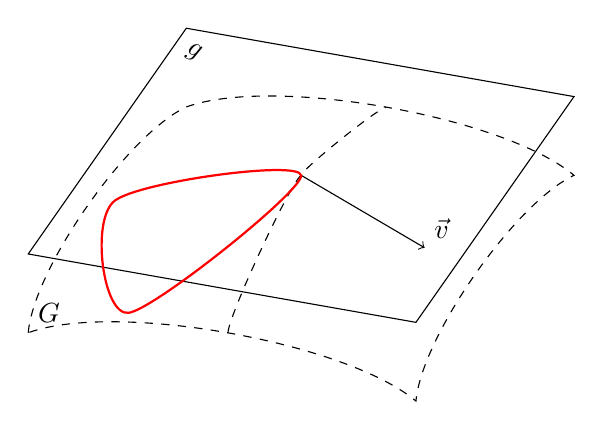
\begin{tikzpicture}[x={(170:1cm)},y={(55:.7cm)},z={(90:1cm)}]
  \draw (2.5,-2.5,0) -- (2.5,2.5,0) -- (-2.5,2.5,0) -- (-2.5,-2.5,0) -- cycle;
  \draw[dashed,looseness=.6] (2.5,-2.5,-1) node[above right] {$G$}
  to[bend left] (2.5,2.5,-1)
  to[bend left] coordinate (mp) (-2.5,2.5,-1)
  to[bend right] (-2.5,-2.5,-1)
  to[bend right] coordinate (mm) (2.5,-2.5,-1)
  -- cycle;
  \draw[dashed,looseness=.2] (mm) to[bend left] (0,0,0) to[bend left] (mp);

  \draw[->] (0,0,0) -- (-2,-1,0) node[above right] {$\vec v$};
  \draw[red, thick] plot [smooth cycle]  coordinates {(0, 0, 0) (1, -3, -0.2) (2, -1, -0.1)};
  \draw (2.5,2.5,0) node[below right, rotate=-25] {$\mathfrak{g}$};
\end{tikzpicture}
\caption{Lie Group and Associated Lie Algebra}
\label{fig:1}
\end{figure}

\noindent
These definitions aren't the most intuitive, so I provide Figure \ref{fig:1} to help the reader see the geometric interpretations. We let $G$ be a Lie Group and $\mathfrak{g}$ be a Lie Algebra, or a tangent space to the manifold, or Lie Group. Lie Algebras are tangent space to the lie group at the identity. Let $G$ be a lie group, then the $T_e G$ (tangent space at the identity) is an interesting vector space with a remarkable structure called the lie algebra structure. We now will prove a few results relating to this structure and the define the Lie Algebra using the bilinear map called the Lie Bracket,

\begin{nlemma}
  Let $G$ be a matrix lie group, and $g \in G$, then,
  $$ \xi \in T_eG \implies g\xi g^{-1} \in T_eG $$
\end{nlemma}
\noindent
\textbf{Note:} $g \xi g^{-1}$ is a matrix expression.\\

\begin{proof}
  Let $c(t) \in G$ be a curve in $G$, such that $c(0) = e$ and $\dot c (0) = \xi$. Define $\g (t) = gc(t)g^{-1}$. Then $\g(0) = g c(0) g^{-1} = e$ and $\dot\g (0) = g \dot c (0) g^{-1} = g\xi g^{-1} \in T_e G$.
\end{proof}

\begin{nprop}
  Let $G$ be a matrix lie group and $\xi, \eta \in T_eG$. Then, $\xi\eta - \eta\xi \in T_eG$
\end{nprop}
\begin{proof}
  Let $c(t) \in G$ be a curve such that $c(0) = e$ and $\dot c(0) = \xi$ also define $b(t) = c(t)\eta c(t)^{-1} \in T_eG$ by Lemma 1.5. Then $\dot b(t) \in T_eG$.
  \begin{align*}
    \dot b(0) &= \dot c(0)\eta c(0)^{-1} + c(0)\eta + \di {c(t)} t (0)\\
    &= \dot c(0)\eta c(0)^{-1} - c(0)\eta c(0)^{-1}\dot c(0) c(0)^{-1}\\
    &= \xi \eta - \eta\xi
  \end{align*}
  As $\dot b(t) \in T_eG$, then $\xi \eta - \eta\xi \in T_eG$
\end{proof}

\noindent
Now we have a Lie Algebra,
\begin{ndefi}[Lie Algebra]
  A lie algebra is a vector space endowed with a {commutator }(or Lie bracket), that is a bilinear map. If we have,
  $$ [\cdot,\, \cdot] : V \times V \to V $$
  such that,
  \begin{itemize}
    \item $[B,\, A] = - [A,\, B]$ (skew-symmetry property)
    \item $[[A,\, B], C] + [[B,\, C], A] + [[C,\, A],\, B] = 0 \quad \fa A, B, C \in V \qquad$ (Jacobi Identity)
  \end{itemize}
\end{ndefi}

\noindent
The Lie Bracket, could be any bilinear map and the behaviour of this map is related to the space that we are considering. In particular, when we consider the matrix lie groups, we are interested in the Lie Bracket defined in Theorem \refeq{ref:LBthm}

\begin{nthm}\label{ref:LBthm}
  Let $G$ be a matrix Lie group. Then $T_eG$ is a lie algebra with bracket given by the matrix commutator. Denoted by $\mathfrak{g}$.
  $$ [A,\, B] = AB - BA $$
\end{nthm}
